\setlength{\baselineskip}{20pt}
\chapter{面向无额外推理成本的特征增强算法研究}
\label{cha:chap3}

本章针对判别式骨干网络提取的特征中仍残留噪声这一共性问题，提出一种面向无额外推理成本的特征增强算法。该算法的核心思想是将扩散模型的去噪过程与骨干网络的特征提取过程进行统一建模，并通过参数融合机制在推理阶段完全消除去噪操作带来的额外计算开销。本章首先在第\ref{sec:chap3_problem}节阐述研究问题并给出整体框架设计；随后在第\ref{sec:chap3_joint}节详细介绍联合特征提取与特征去噪的建模方法；接着在第\ref{sec:chap3_fusion}节推导特征提取与去噪的参数融合算法及其数学等价性证明；第\ref{sec:chap3_exp_setup}节和第\ref{sec:chap3_exp_result}节分别介绍实验设置与实验结果分析；最后在第\ref{sec:chap3_summary}节对本章工作进行总结。

\section{研究问题与整体框架设计}
\label{sec:chap3_problem}

如第一章所述，判别式视觉模型通过骨干网络逐层提取特征表示，并在此基础上完成分类、检测、分割和检索等下游任务\cite{6472238}。然而，在实际推理过程中，骨干网络输出的特征向量中不可避免地包含来自多种来源的噪声：一方面，输入图像本身可能受到光照变化、遮挡、背景杂乱和传感器噪声等因素的干扰；另一方面，特征在网络逐层传播的过程中也会累积表示噪声，导致最终特征的类内分布发散、类间边界模糊，进而影响下游任务的判别精度。

扩散模型\cite{sohl2015deep,ho2020denoising}作为一类强大的生成式框架，具备经过充分验证的噪声去除能力——通过迭代的噪声估计与去除过程，能够从含噪数据中逐步恢复原始的干净分布\cite{10419041}。然而，将扩散模型的去噪能力直接应用于判别式任务面临两个核心矛盾：其一，标准扩散模型的去噪过程需要在特征提取完成之后附加一个独立的多步迭代去噪模块，这将引入不可忽视的额外推理延迟；其二，若为每个下游任务单独设计扩散去噪流程（如DiffusionDet\cite{chen2023diffusiondet}对检测框去噪、DiffSeg\cite{tian2023diffuse}对分割图去噪），则方法缺乏通用性，难以在不同任务间迁移。

\begin{figure}[htbp]
    \centering
    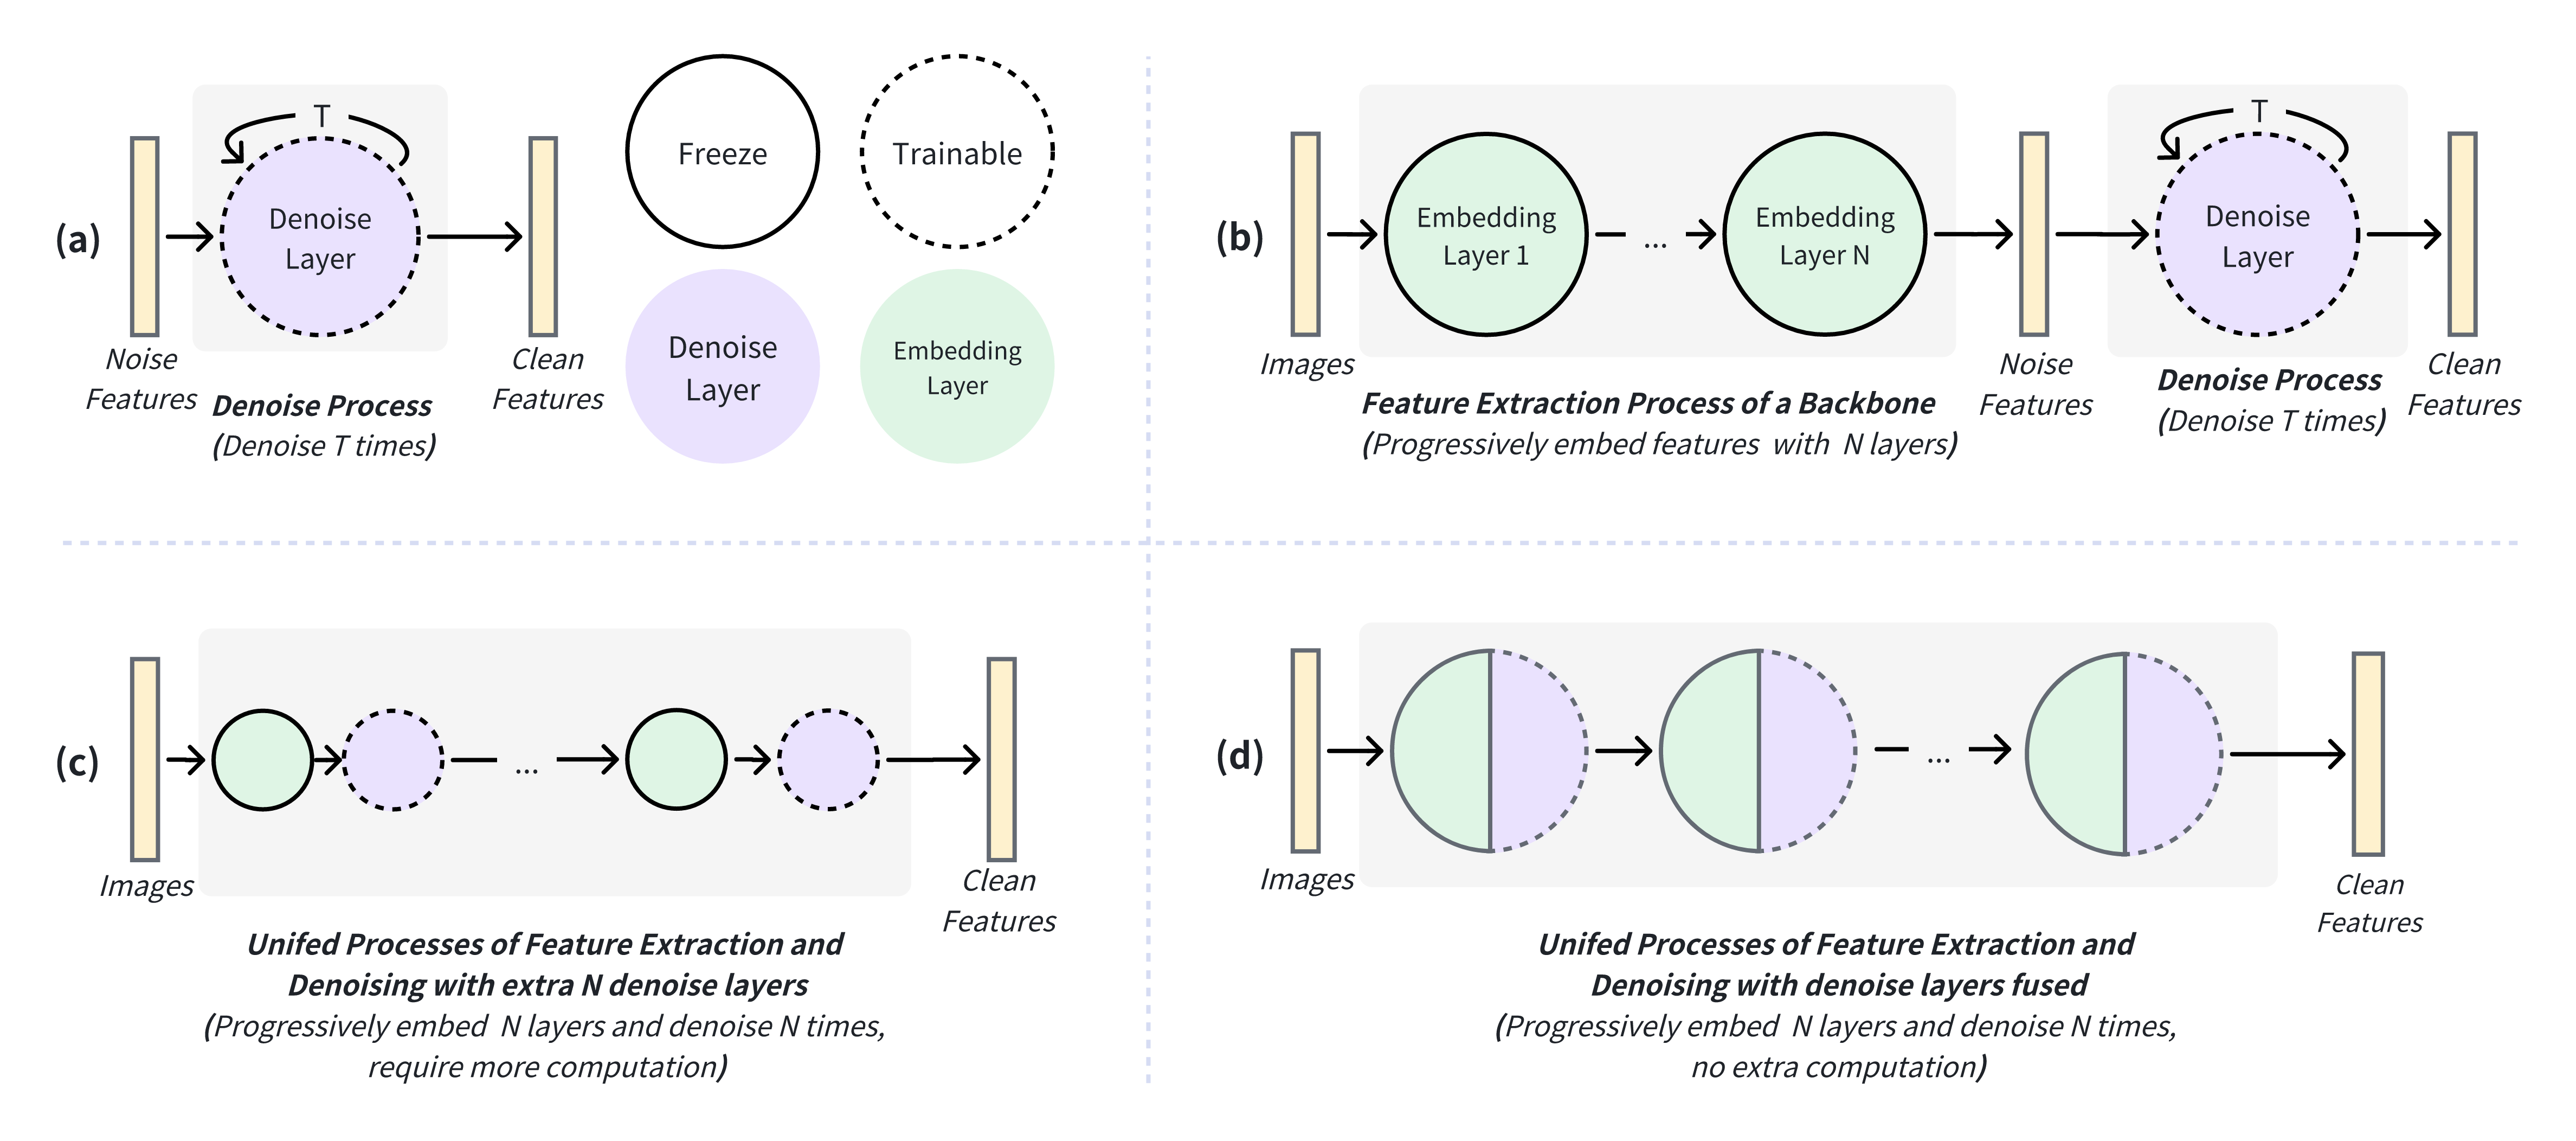
\includegraphics[width=0.95\textwidth]{figures/intro5.png}
    \caption{特征去噪与特征提取统一框架的思路演进示意图\protect\\[-2pt]{\rm Fig.\;\thefigure\quad Illustration of the idea evolution from separate denoising to unified feature extraction and denoising framework}}\label{fig:intro_evolution}
\end{figure}

为解决上述矛盾，本章提出了一种将特征提取与特征去噪统一建模的算法框架\cite{xu2024denoiserep}。其核心思路如图\ref{fig:intro_evolution}所示，经历了从分离到统一、从额外开销到零开销的四个阶段的演进：

（a）标准去噪过程：去噪层对含噪特征执行$T$步迭代去噪以获得干净特征，这是扩散模型的基本工作模式。

（b）骨干网络末端附加去噪：在判别式骨干网络的$N$个嵌入层完成特征提取之后，在网络末端附加一个独立的去噪模块对输出特征进行$T$步去噪。这种方式虽然能够改善特征质量，但去噪模块作为独立组件引入了额外的推理延迟。

（c）逐层统一但增加计算：将去噪层嵌入骨干网络的每一个特征提取层，使特征提取与去噪在每一层同步进行。每一层的嵌入操作与去噪操作并行执行，实现了特征提取与去噪的统一。然而，由于每一层新增了独立的去噪分支，总体计算量相应增加。

（d）参数融合实现零额外开销：在方案（c）的基础上，通过数学推导证明去噪层的参数可以与对应嵌入层的参数进行等价融合。融合后的网络结构和参数量与原始骨干网络完全相同，从而在推理阶段实现了特征去噪的零额外计算开销。这是本章算法的最终方案。

基于上述思路，本章所提方法的整体框架可以概括为三个阶段。第一阶段，冻结预训练骨干网络的全部参数，仅训练附加在每一层上的轻量级去噪模块；第二阶段，利用扩散过程对每一层输出的特征进行加噪，并训练对应的去噪模块学习预测添加的噪声；第三阶段，在推理时将训练好的去噪模块参数与原始嵌入层参数进行融合，获得增强后的网络参数。该方法不依赖任何标签信息，可以在无监督条件下完成训练，且适用于ResNet\cite{he2016deep}、ViT\cite{dosovitskiy2020image}、Swin Transformer\cite{liu2021swin}和VMamba\cite{liu2024vmamba}等多种骨干网络架构。

\section{联合特征提取与特征去噪}
\label{sec:chap3_joint}

本节详细介绍如何将扩散模型的去噪机制融入判别式骨干网络的特征提取过程中，构建联合特征提取与特征去噪的统一框架。

\subsection{扩散过程建模}

本方法借鉴扩散模型的基本框架\cite{ho2020denoising}，在特征空间上构建前向扩散过程。与传统扩散模型在像素空间上操作不同，本方法以骨干网络各层输出的特征向量作为数据样本进行扩散建模。

设骨干网络包含$N$个级联的嵌入层，第$i$层输出的特征向量记为$F_i$（$i = 1, 2, \ldots, N$）。对于每一层的特征$F_i$，通过不断添加高斯噪声来模拟其特征分布的前向扩散过程：
\begin{equation}
q(\mathbf{x}_{1:T} | \mathbf{x}_0) \triangleq \prod_{t=1}^T q(\mathbf{x}_t | \mathbf{x}_{t-1})
\label{eq:chap3_forward_joint}
\end{equation}
\vspace{-2pt}
\begin{equation}
q(\mathbf{x}_t|\mathbf{x}_{t-1}) \triangleq \mathcal{N}\!\left(\mathbf{x}_t;\, \sqrt{1-\beta_t}\,\mathbf{x}_{t-1},\, \beta_t \mathbf{I}\right)
\label{eq:chap3_forward_step}
\end{equation}
其中$\mathbf{x}_0$表示骨干网络某一层输出的特征向量$F_i$，$t$表示扩散步数，$\beta_t$为预先设定的噪声调度参数，$\mathbf{x}_t$表示经过$t$步扩散后获得的含噪样本。利用扩散过程的重参数化性质，可以直接从$\mathbf{x}_0$一步获得任意步数$t$对应的含噪样本：
\begin{equation}
\mathbf{x}_t = \sqrt{\bar{a}_t}\,\mathbf{x}_0 + \sqrt{1-\bar{a}_t}\,\boldsymbol{\epsilon}, \quad \boldsymbol{\epsilon} \sim \mathcal{N}(\mathbf{0},\, \mathbf{I})
\label{eq:chap3_reparam}
\end{equation}
其中$a_t = 1 - \beta_t$，$\bar{a}_t = \prod_{s=1}^{t} a_s$为累积噪声调度系数。

在推理阶段，对骨干网络输出的特征执行$T$步反向去噪，以获得更干净、更具判别性的特征表示：
\begin{equation}
p_\theta(\mathbf{x}_{0:T}) \triangleq p(\mathbf{x}_T)\prod_{t=1}^T p_\theta(\mathbf{x}_{t-1}|\mathbf{x}_t)
\label{eq:chap3_reverse_joint}
\end{equation}
\vspace{-2pt}
\begin{equation}
p_\theta(\mathbf{x}_{t-1}|\mathbf{x}_t) \triangleq \mathcal{N}\!\left(\mathbf{x}_{t-1};\, \boldsymbol{\mu}_\theta(\mathbf{x}_t, t),\, \boldsymbol{\Sigma}_\theta(\mathbf{x}_t, t)\right)
\label{eq:chap3_reverse_step}
\end{equation}
其中$\mathbf{x}_T$表示推理阶段骨干网络输出的含噪特征，$T$为去噪步数，控制去噪的幅度。通过$p_\theta(\mathbf{x}_{t-1}|\mathbf{x}_t)$逐步去噪，最终获得去噪后的干净特征$\mathbf{x}_0$。可以根据不同数据集和骨干网络的特点，调节$t$的大小以获得最优的去噪效果。

\subsection{去噪网络训练}

本方法的一个关键设计是将骨干网络的$N$个级联嵌入层重新解释为$N$步递归去噪过程。具体而言，为骨干网络的每一个嵌入层附加一个轻量级的去噪模块$D_i(\cdot)$（$i = 1, 2, \ldots, N$），在训练阶段冻结骨干网络的原始参数，仅优化这些去噪模块的参数。

训练过程的具体步骤如算法\ref{alg:training_chap3}所示。对于第$i$层，根据其在网络中的深度位置设定对应的扩散步数$t = i$，即浅层对应较小的噪声幅度，深层对应较大的噪声幅度。这一设计的直觉在于：随着特征在网络中逐层传播，累积的噪声逐渐增加，因此深层需要更强的去噪能力。对每一层的特征$F_i$，首先按式（\ref{eq:chap3_reparam}）进行前向扩散获得含噪样本$\mathbf{x}_t$，然后训练去噪模块$D_i$学习预测添加的噪声$\boldsymbol{\epsilon}$，优化目标为最小化预测噪声与真实噪声之间的均方误差：
\begin{equation}
\mathcal{L}_p = \sum_{i=1}^{N}\left\|\boldsymbol{\epsilon}_i - D_{\theta_i}(\mathbf{x}_{t_i},\, t_i)\right\|^2
\label{eq:chap3_denoise_loss}
\end{equation}
其中$\boldsymbol{\epsilon}_i$为第$i$层采样的真实噪声，$D_{\theta_i}(\mathbf{x}_{t_i}, t_i)$为第$i$个去噪模块对噪声的预测。

\begin{algorithm}[htbp]
\caption{特征去噪模块训练算法}
\label{alg:training_chap3}
\begin{algorithmic}[1]
\REQUIRE 骨干网络嵌入层数$N$，各层提取的特征$\{F_i\}_{i=1}^{N}$，待训练的去噪模块$\{D_i(\cdot)\}_{i=1}^{N}$。
\REPEAT
\FOR {每一层 $i \in [N, 1]$}
\STATE $t = i$：根据层的顺序指定当前层的扩散步数$t$。
\STATE $\boldsymbol{\epsilon} \sim \mathcal{N}(\mathbf{0}, \mathbf{I})$：随机采样一个高斯噪声。
\STATE $\mathbf{x}_t = \sqrt{\bar{a}_t}F_i + \sqrt{1-\bar{a}_t}\boldsymbol{\epsilon}$：按式（\ref{eq:chap3_reparam}）执行前向扩散。
\STATE 对$\nabla_\theta\|\boldsymbol{\epsilon} - D_i(\mathbf{x}_t, t)\|^2$执行梯度下降步。
\ENDFOR
\UNTIL{收敛}
\end{algorithmic}
\end{algorithm}

值得指出的是，本方法的训练过程完全不依赖标签信息，因为去噪目标函数式（\ref{eq:chap3_denoise_loss}）本质上是一个生成式建模目标——通过学习特征的分布来实现去噪，无需任何标注信息的参与。这意味着该方法可以利用大量无标签数据进行训练，具有良好的实用性。同时，该方法也兼容有监督学习范式：当标签可用时，可以将任务特定的有监督损失$\mathcal{L}_l$与去噪损失$\mathcal{L}_p$进行加权组合：
\begin{equation}
\mathcal{L} = (1-\lambda)\,\mathcal{L}_l + \lambda\,\mathcal{L}_p
\label{eq:chap3_total_loss}
\end{equation}
其中$\lambda$为平衡两个损失项的权重系数。实验结果表明，引入标签信息能够进一步提升特征增强的效果。

\section{特征提取与去噪的参数融合}
\label{sec:chap3_fusion}

上一节所述的联合特征提取与去噪框架虽然能够有效提升特征的判别性，但在推理阶段需要额外执行去噪层的前向计算，引入了不可忽视的推理延迟。本节提出一种参数融合策略，将去噪层的参数合并至对应嵌入层的参数中，从理论上证明融合前后的数学等价性，从而在推理阶段完全消除额外开销。

\subsection{双分支结构设计}

\begin{figure}[htbp]
    \centering
    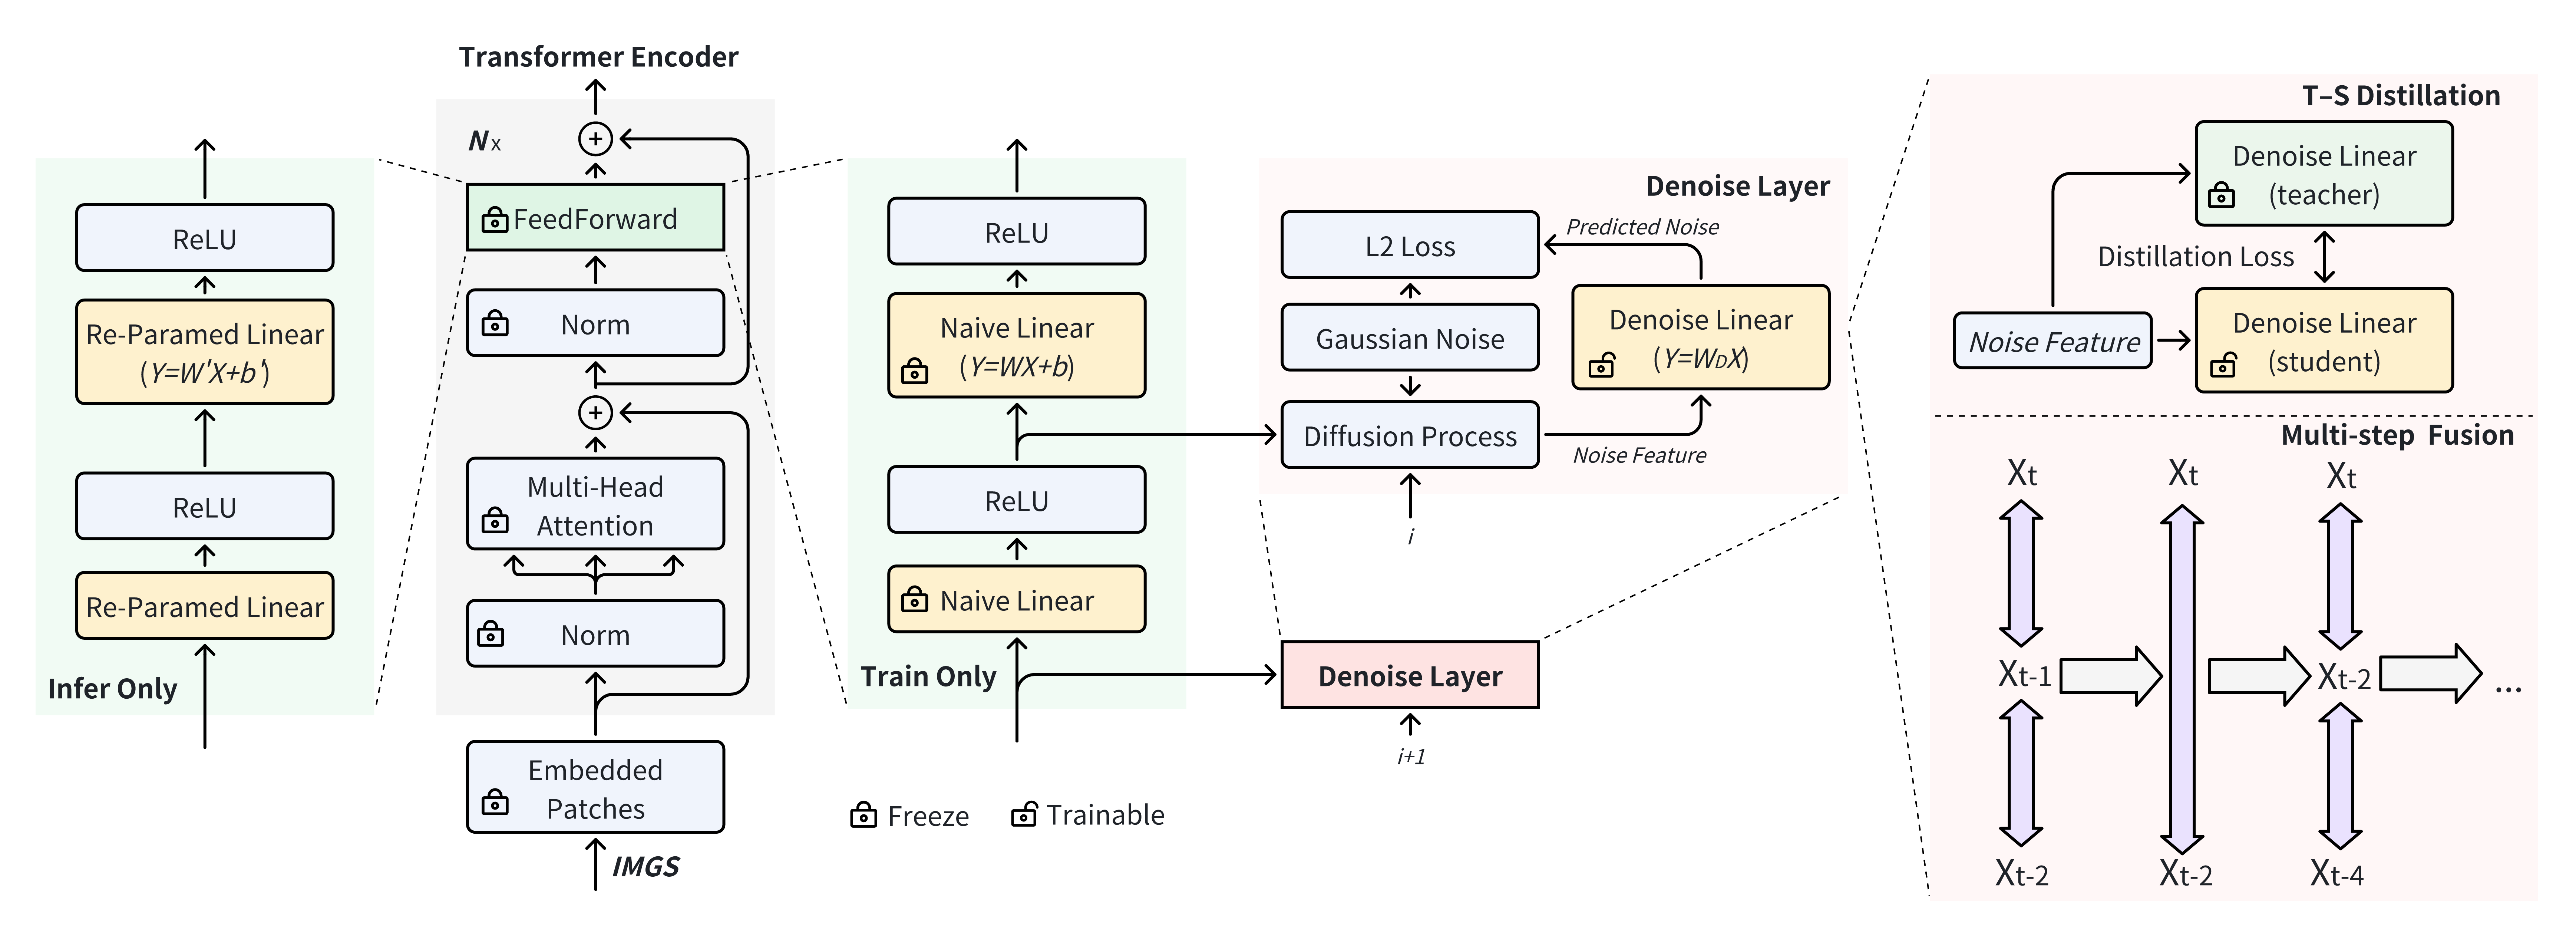
\includegraphics[width=0.95\textwidth]{figures/train2.png}
    \caption{本章所提方法的训练与推理流程示意图\protect\\[-2pt]{\rm Fig.\;\thefigure\quad Pipeline of the proposed method for training and inference}}\label{fig:train_pipeline}
\end{figure}

如图\ref{fig:train_pipeline}所示，本方法将骨干网络（以Vision Transformer为例）中每一个Transformer编码层的线性层扩展为双分支结构：一个分支为原始的嵌入层（执行特征提取），另一个分支为新增的去噪层（执行特征去噪）。

在训练阶段（图\ref{fig:train_pipeline}右侧``Train Only''部分），骨干网络的原始参数被冻结，仅训练新增的去噪层参数。去噪层的训练方法与第\ref{sec:chap3_joint}节描述一致：将每一层的特征通过扩散过程加噪后，送入对应的去噪层进行噪声预测训练。图\ref{fig:train_pipeline}右上方展示了教师--学生蒸馏和多步融合机制，这两项增强策略将在第四章中详细阐述。

在推理阶段（图\ref{fig:train_pipeline}左侧``Infer Only''部分），通过参数重参数化技术，将双分支结构合并为单分支结构。具体而言，将原始嵌入层参数$W$替换为融合后的参数$W'$，其中$W'$同时包含了特征提取和特征去噪的功能，但参数量与原始的$W$完全相同。这种设计思路借鉴了结构重参数化的理念\cite{ding2021repvgg}——在训练阶段使用更丰富的多分支结构以增强表达能力，在推理阶段将其融合为单一结构以保持高效。

需要指出的是，虽然本节以Transformer架构为例进行说明，但所提方法同样适用于CNN架构。只要骨干网络的嵌入层可以表示为线性变换$Y = WX + b$的形式，本方法的参数融合策略即可直接应用。

\subsection{参数融合数学推导}

本小节给出从一步去噪到参数融合的完整数学推导，证明融合前后的严格等价性。

根据DDPM\cite{ho2020denoising}的反向去噪公式，对特征的一步去噪过程可以表示为：
\begin{equation}
\mathbf{x}_{t-1} = \frac{1}{\sqrt{a_t}}\!\left(\mathbf{x}_t - \frac{1-a_t}{\sqrt{1-\bar{a}_t}}\,D_\theta(\mathbf{x}_t,\, t)\right) + \sigma_t\,\mathbf{z}
\label{eq:chap3_one_step_denoise}
\end{equation}
其中$a_t = 1 - \beta_t$，$D_\theta$为去噪网络的参数，$\sigma_t$为噪声系数，$\mathbf{z} \sim \mathcal{N}(\mathbf{0}, \mathbf{I})$。

设骨干网络某一嵌入层的线性变换为$Y = WX + b$，其中$W$和$b$分别为该层的权重矩阵和偏置向量。将式（\ref{eq:chap3_one_step_denoise}）进行变换，并同时左乘$W$，可以得到：
\begin{equation}
\frac{1}{\sqrt{a_t}}\,Y_t - Y_{t-1} = \frac{1-a_t}{\sqrt{a_t}\,\sqrt{1-\bar{a}_t}}\,D_\theta\, Y_t - \sigma_t\,\mathbf{z}
\label{eq:chap3_transform}
\end{equation}
将$Y_t = WX_t + b$代入并整理，可以获得一步去噪与线性变换合并后的简化形式：
\begin{equation}
\left\{\;\begin{aligned}
Y_{t-1} &= \bigl[W - C_1(t)\,W W_D\bigr]\,X_t + W\,C_2(t)\,C_3 + b \\[4pt]
C_1(t) &= \frac{1-a_t}{\sqrt{a_t}\,\sqrt{1-\bar{a}_t}} \\[4pt]
C_2(t) &= \frac{1-\bar{a}_{t-1}}{1-\bar{a}_t}\,\beta_t \\[4pt]
C_3 &= \mathbf{z} \sim \mathcal{N}(\mathbf{0},\, \mathbf{I})
\end{aligned}\right.
\label{eq:chap3_combined}
\end{equation}
其中$W_D$为去噪模块$D_\theta(\mathbf{x}_t, t)$的参数矩阵，$X_t$为该线性层的输入，$Y_t$为原始线性层的输出，$Y_{t-1}$为经过一步去噪后的输出。

式（\ref{eq:chap3_combined}）揭示了参数融合的核心思想：在推理阶段，可以将原始参数$W$替换为融合后的参数：
\begin{equation}
W' = W - C_1(t)\,W W_D
\label{eq:chap3_w_prime}
\end{equation}
\vspace{-2pt}
\begin{equation}
b' = W\,C_2(t)\,C_3 + b
\label{eq:chap3_b_prime}
\end{equation}
从而将特征提取操作$Y = WX + b$与一步去噪操作统一为$Y_{t-1} = W'X_t + b'$。融合后的$W'$与原始$W$具有相同的维度，因此不引入任何额外的参数量和计算量。这是一种零额外推理开销的特征增强策略。

由于骨干网络中各层之间存在级联关系，不同层设置不同的$t$值。根据算法\ref{alg:inference_chap3}的设计，第$i$层使用$t = i$，使得级联的$N$个嵌入层的逐层一步去噪（每层完成$Y_t \rightarrow Y_{t-1}$）等价于完整的$N$步去噪过程（$Y_N \rightarrow Y_0$），从而保证了去噪过程的连续性。

\begin{algorithm}[htbp]
\caption{参数融合推理算法}
\label{alg:inference_chap3}
\begin{algorithmic}[1]
\REQUIRE 骨干网络嵌入层数$N$，各层特征$\{F_i\}_{i=1}^{N}$，已训练的去噪模块参数$\{W_{D_i}\}_{i=1}^{N}$，骨干网络预训练参数$\{W_i\}_{i=1}^{N}$和$\{b_i\}_{i=1}^{N}$。
\ENSURE 去噪后的特征$F^0$。
\FOR {每一层 $i \in [N, 1]$}
\STATE $t = i$：根据当前层的深度设定去噪幅度。
\STATE $W' = \left[W_i - C_1(t)W_iW_{D_i}\right]$，$b' = W_iC_2(t)C_3 + b_i$：按式（\ref{eq:chap3_w_prime}）--（\ref{eq:chap3_b_prime}）进行参数融合。
\STATE $F^{t-1} = W'F^t + b'$：融合特征提取与特征去噪。
\ENDFOR
\STATE \textbf{返回} $F^0$
\end{algorithmic}
\end{algorithm}

进一步地，若需要增大单层的去噪幅度，可以将一步去噪扩展为两步去噪。以下给出两步去噪的推导过程。对$Y_t$的一步去噪为：
\begin{equation}
\frac{1}{\sqrt{a_t}}\,Y_t - Y_{t-1} = C_1(t)\,D_\theta\, Y_t - \sigma_t\,\mathbf{z}
\label{eq:chap3_two_step_1}
\end{equation}
对$Y_{t-1}$的一步去噪为：
\begin{equation}
\frac{1}{\sqrt{a_{t-1}}}\,Y_{t-1} - Y_{t-2} = C_1(t\!-\!1)\,D_\theta\, Y_{t-1} - \sigma_{t-1}\,\mathbf{z}
\label{eq:chap3_two_step_2}
\end{equation}
通过消去$Y_{t-1}$并将$Y_t = WX_t + b$代入，可得两步去噪的融合公式：
\begin{equation}
\left\{\;\begin{aligned}
Y_{t-2} &= W''X_t + C'' \\[6pt]
W'' &= \frac{1}{\sqrt{a_{t-1}}}\!\left\{\frac{W}{\sqrt{a_t}} - \bigl[C_1(t) + C_1(t\!-\!1)\bigr]\,WW_D + \sqrt{a_t}\,C_1(t\!-\!1)\,C_1(t)\,WW_DW_D\right\} \\[6pt]
C'' &= \frac{1}{\sqrt{a_{t-1}}}\!\left[W\,C_2(t) + \sqrt{a_t}\,W\,C_2(t\!-\!1) - \sqrt{a_t}\,C_1(t\!-\!1)\,C_2(t)\,WW_D\right]\mathbf{z} + b
\end{aligned}\right.
\label{eq:chap3_two_step_combined}
\end{equation}
上述推导表明，单个嵌入层可以完成两步去噪，且其结果仍然可以通过参数融合表示为一次线性变换。此时为保证整体去噪过程的连续性，各层的$t$值应按步长2递减。这一扩展机制使得去噪幅度可以根据实际需求灵活调节。

本章所提的算法基于特征级别的去噪，能够迁移至各类下游判别式任务。该算法在每一层上对特征进行去噪，能够更好地去除各阶段的噪声——因为推理阶段的噪声来自多个方面，既可能是输入图像中的噪声，也可能是在网络传播过程中产生的噪声。逐层去噪避免了噪声的累积效应，从而获得更高质量的特征输出。此外，可以通过控制$t$、$\beta_t$和去噪步数来调节去噪强度，以适应不同应用场景中数据的噪声特性，体现了良好的通用性和灵活性。

\section{本章实验设计}
\label{sec:chap3_exp_setup}

\subsection{实验设置与评价指标}

为全面验证本章所提方法的有效性和通用性，分别在行人重识别、图像分类、目标检测和图像分割四类判别式视觉任务上进行实验评估。

在行人重识别任务中，选取四个广泛使用的基准数据集：DukeMTMC-reID\cite{zheng2017unlabeled}、Market-1501\cite{zheng2015scalable}、MSMT17\cite{wei2018person}和CUHK-03\cite{li2014deepreid}。这四个数据集涵盖了行人重识别中多种典型的挑战场景，包括跨摄像头视角变化、背景干扰和姿态差异等。评价指标采用平均精度均值（mean Average Precision, mAP）和Rank-1准确率。mAP综合衡量检索结果在所有查询上的平均精度，Rank-1表示检索结果中排名最高的图像为正确匹配的概率。所有结果基于单查询设定。

在图像分类任务中，选取大规模通用分类数据集ImageNet-1k\cite{deng2009imagenet}以及三个细粒度分类数据集CUB200\cite{wah2011caltech}、Oxford-Pet\cite{parkhi2012cats}和Flowers\cite{nilsback2008automated}。ImageNet-1k包含1000个类别、超过120万张训练图像，是验证分类模型通用能力的标准基准。三个细粒度数据集分别聚焦鸟类、宠物和花卉的细粒度类别识别。评价指标采用Top-1准确率和Top-5准确率。

在目标检测任务中，选取COCO\cite{karpathy2015deep}数据集。COCO是目标检测领域最常用的大规模基准，包含80个目标类别和超过11万张训练图像。评价指标采用平均精度（AP）及其在不同IoU阈值下的变体AP$_{50}$和AP$_{75}$。

在图像分割任务中，选取ADE20K\cite{zhou2017scene}数据集。ADE20K包含约2万张图像和150个语义类别，广泛用于语义分割模型的评估。评价指标采用平均交并比（mIoU）和边界交并比（B-IoU）。

\subsection{实现细节与训练策略}

所有实验在配备两块NVIDIA RTX 3090 GPU的服务器上进行，处理器为Intel Xeon Gold 5218R（2.10GHz）。训练轮次设为120个epoch，初始学习率设为0.0004，训练阶段的批量大小为64，推理阶段的批量大小为256，扩散步数$t$设为1000。

在训练策略方面，为了更好地约束去噪特征对下游任务的适配性，采用交替微调的训练方式。具体而言，本方法的参数与基线模型的参数交替训练：当训练一部分参数时，冻结其余参数进行微调，每次微调10个epoch，总轮次为120个epoch。在评估时，对相同设置下的实验进行5次独立运行并取平均值，以确保实验结果的可靠性。

\section{实验结果与分析}
\label{sec:chap3_exp_result}

\subsection{基础效果与对比分析}

本节首先验证所提方法在多个判别式任务上的基础有效性，然后与现有先进方法进行对比分析。

表\ref{tab:chap3_multi_task}展示了本章方法在四类代表性判别式任务上的实验结果。可以看到，在不增加任何模型参数的前提下，所提方法在图像分类、行人重识别、目标检测和图像分割四个任务上均取得了稳定且显著的性能提升。

\begin{table}[htbp]
\centering
\caption{本章方法在多种判别式任务上的实验结果\protect\\[-2pt]{\rm Table\;\thetable\quad Experimental results on multiple discriminative tasks}}\label{tab:chap3_multi_task}
\vspace{0.2cm}
\renewcommand{\arraystretch}{1.2}
\begin{tabular}{lcccccc}
\hline \hline
任务 & 模型 & 骨干网络 & 数据集 & 指标 & 基线 & +本章方法 \\
\hline
分类 & SwinT & SwinV2-T & ImageNet-1k & acc@1 & 81.82\% & 82.13\% \\
检索 & TransReID-SSL & ViT-S & MSMT17 & mAP & 66.30\% & 67.33\% \\
检测 & Mask-RCNN & Swin-T & COCO & AP & 42.80\% & 44.30\% \\
分割 & FCN & ResNet-50 & ADE20K & BIoU & 28.70\% & 29.90\% \\
\hline\hline
\end{tabular}
\end{table}

接下来，本节分析标签信息对本方法性能的影响。如第\ref{sec:chap3_joint}节所述，本方法本质上是一种无标签的去噪训练方式，但也可以在标签可用时通过引入有监督损失来进一步提升性能。表\ref{tab:chap3_label}展示了在TransReID-SSL（ViT-small骨干网络）上的对比实验结果。

\begin{table}[htbp]
\centering
\caption{标签信息对本章方法性能的影响分析\protect\\[-2pt]{\rm Table\;\thetable\quad Analysis of the effect of label information}}\label{tab:chap3_label}
\vspace{0.2cm}
\renewcommand{\arraystretch}{1.2}
\begin{tabular}{lcccc}
\hline \hline
\multirow{2}{*}{方法} & DukeMTMC & MSMT17 & Market1501 & CUHK-03 \\
 & mAP(\%) & mAP(\%) & mAP(\%) & mAP(\%) \\
\hline
TransReID-SSL（基线） & 81.20 & 66.30 & 91.20 & 83.50 \\
+本章方法（无标签） & 81.72 & 66.87 & 91.82 & 83.72 \\
+本章方法（有标签） & 82.12 & 67.33 & 92.05 & 84.11 \\
+本章方法（合并数据集） & 81.78 & 66.99 & 91.80 & 83.86 \\
\hline\hline
\end{tabular}
\end{table}

从表\ref{tab:chap3_label}中可以得出以下三点结论：

（1）无标签训练的有效性。与基线方法（第1行）相比，在无标签条件下添加本章所提方法（第2行）即可在四个数据集上分别获得0.52\%、0.57\%、0.62\%和0.22\%的mAP提升，验证了该方法确实具备对特征的有效去噪能力。

（2）标签信息的互补性。引入标签信息进行有监督训练（第3行）后，相比无标签版本在四个数据集上进一步获得0.32\%$\sim$0.70\%的mAP提升，表明该去噪方法具有良好的标签兼容性，无论在有监督还是无监督条件下均能有效提升特征质量。

（3）跨数据集泛化能力。将四个数据集合并进行无标注训练（第4行），其性能优于在单个数据集上训练的无标签版本（第2行），说明引入更多无标签数据可以进一步增强去噪模块的泛化能力，印证了该方法良好的可扩展性。

进一步地，表\ref{tab:chap3_reid_sota}展示了本方法与当前先进行人重识别方法的对比结果。

\begin{table*}[htbp]
\centering
\caption{与先进行人重识别方法的对比实验\protect\\[-2pt]{\rm Table\;\thetable\quad Comparison with state-of-the-art ReID methods}}\label{tab:chap3_reid_sota}
\vspace{0.2cm}
\renewcommand{\arraystretch}{1.15}
\begin{tabular}{llcccccccc}
\hline \hline
\multirow{2}{*}{方法} & \multirow{2}{*}{骨干网络} & \multicolumn{2}{c}{MSMT17} & \multicolumn{2}{c}{Market1501} & \multicolumn{2}{c}{DukeMTMC} & \multicolumn{2}{c}{CUHK03-L} \\
 & & mAP & R1 & mAP & R1 & mAP & R1 & mAP & R1 \\
\hline
MGN\cite{wang2018learning} & ResNet-50 & -- & -- & 86.90 & 95.70 & 78.40 & 88.70 & 67.40 & 68.00 \\
OSNet\cite{zhou2019omni} & OSNet & 52.90 & 78.70 & 84.90 & 94.80 & 73.50 & 88.60 & -- & -- \\
BAT-net\cite{fang2019bilinear} & GoogLeNet & 56.80 & 79.50 & 87.40 & 95.10 & 77.30 & 87.70 & 76.10 & 78.60 \\
ABD-Net\cite{chen2019abd} & ResNet-50 & 60.80 & 82.30 & 88.30 & 95.60 & 78.60 & 89.00 & -- & -- \\
RGA-SC\cite{zhang2020relation} & ResNet-50 & 57.50 & 80.30 & 88.40 & 96.10 & -- & -- & 77.40 & 81.10 \\
ISP\cite{zhu2020identity} & HRNet-W32 & -- & -- & 88.60 & 95.30 & 80.00 & 89.60 & 74.10 & 76.50 \\
CDNet\cite{li2021combined} & CDNet & 54.70 & 78.90 & 86.00 & 95.10 & 76.80 & 88.60 & -- & -- \\
Nformer\cite{wang2022nformer} & ResNet-50 & 59.80 & 77.30 & 91.10 & 94.70 & 83.50 & 89.40 & 78.00 & 77.20 \\
TransReID\cite{He_2021_ICCV} & ViT-base & 61.80 & 81.80 & 87.10 & 94.60 & 79.60 & 89.00 & 82.30 & 84.60 \\
TransReID-SSL\cite{luo2021self} & ViT-small & 66.30 & 84.80 & 91.20 & 95.80 & 81.20 & 87.80 & 83.50 & 85.90 \\
TransReID-SSL & ViT-base & 75.00 & 89.50 & 93.10 & 96.52 & 84.10 & 92.60 & 87.80 & 89.20 \\
CLIP-ReID\cite{li2023clip} & ViT-base & 75.80 & 89.70 & 90.50 & 95.40 & 83.10 & 90.80 & -- & -- \\
\hline
TransReID +本章方法 & ViT-base & 62.23 & 82.02 & 87.25 & 94.63 & 80.12 & 89.33 & 82.44 & 84.61 \\
TransReID-SSL +本章方法 & ViT-small & 67.33 & 85.50 & 92.05 & 96.68 & 82.12 & 88.72 & 84.11 & 86.47 \\
TransReID-SSL +本章方法 & ViT-base & 75.35 & 89.62 & 93.26 & 96.55 & 84.31 & 92.90 & 88.08 & 89.29 \\
CLIP-ReID +本章方法 & ViT-base & 76.30 & 90.60 & 91.10 & 95.80 & 83.70 & 91.60 & -- & -- \\
\hline \hline
\end{tabular}
\end{table*}

从表\ref{tab:chap3_reid_sota}可以观察到以下规律：

（1）本方法在ViT-base骨干网络上的四个数据集中几乎达到了所有指标的最优性能，表明所提的特征去噪策略能够有效提升当前先进方法的性能上限。

（2）添加本方法后的模型在所有数据集上均优于使用相同骨干网络的原始方法。值得注意的是，小规模骨干网络（ViT-small）添加本方法后的性能提升幅度大于大规模骨干网络（ViT-base）。这一现象的合理解释是：本方法本质上是一种去噪模块，用于去除推理阶段特征中包含的噪声。对于参数量较大的骨干网络，其提取的特征已经具有较好的表达能力，特征中残留的噪声相对较少，因此去噪的提升空间有限。而对于参数量较小、拟合能力有限的骨干网络，其提取的特征在推理阶段包含较多噪声，去噪操作能够获得更显著的改善效果。

（3）本方法具有良好的模型无关性，可以增量式地应用于任意现有骨干网络的每一层，尤其对于性能较弱的骨干网络，去噪增强的效果更为显著。

\subsection{效率与开销验证}

本章方法的一个核心特性是零额外推理开销。本节通过实验验证参数融合的有效性，并对比不同去噪策略的推理效率。表\ref{tab:chap3_efficiency}展示了基于TransReID-SSL（ViT-small骨干网络）的对比实验结果。

\begin{table}[htbp]
\centering
\caption{参数融合性能与推理效率分析\protect\\[-2pt]{\rm Table\;\thetable\quad Analysis of parameter fusion performance and inference efficiency}}\label{tab:chap3_efficiency}
\vspace{0.2cm}
\renewcommand{\arraystretch}{1.15}
\begin{tabular}{l|c|c|c}
\hline \hline
数据集 & 基线 & +末端去噪 & +本章方法 \\
\hline
DukeMTMC & 81.20\% & 81.56\% & 82.12\% \\
MSMT17 & 66.30\% & 66.81\% & 67.33\% \\
Market1501 & 91.20\% & 91.07\% & 92.05\% \\
CUHK-03 & 83.50\% & 83.59\% & 84.11\% \\
\hline
推理时间 & 0.34s & 0.39s (+15\%) & 0.34s (+0\%) \\
\hline \hline
\end{tabular}
\end{table}

从表\ref{tab:chap3_efficiency}中可以得出以下结论：与基线方法相比，在模型末端附加独立的去噪模块（``末端去噪''）能够在一定程度上提升性能，验证了基于特征的去噪确实有效。然而，这种方式也带来了约15\%的额外推理延迟，因为它在模型末端增加了独立的、参数不可融合的去噪层。

采用本章所提方法后，在四个数据集上均获得了更大幅度的提升。这得益于逐层去噪的设计——由于推理阶段的噪声来自多个方面（输入图像噪声和网络传播噪声），在每一层进行去噪可以避免噪声的逐层累积，获得更高质量的特征输出。更重要的是，由于参数融合机制能够将去噪模块的参数合并至原始嵌入层参数中，本方法不引入任何额外的推理延迟，实现了零额外推理开销的特征增强。

为进一步验证实验的公平性，表\ref{tab:chap3_fairness}对比了基线方法和本章方法在相同额外训练轮次下的性能变化。

\begin{table}[htbp]
\centering
\caption{相同训练轮次下的公平性对比实验\protect\\[-2pt]{\rm Table\;\thetable\quad Fairness comparison under the same training epochs}}\label{tab:chap3_fairness}
\vspace{0.2cm}
\renewcommand{\arraystretch}{1.15}
\begin{tabular}{lcccc}
\hline \hline
训练轮次 & 120 & 160 & 200 & 240 \\
\hline
基线 & 81.18\% & 81.19\% & 81.18\% & 81.16\% \\
+本章方法 & 81.18\% & 81.64\% & 82.00\% & 82.12\% \\
\hline \hline
\end{tabular}
\end{table}

实验结果表明，基线方法在增加训练轮次后性能没有显著提升，甚至略有下降（过拟合），而添加本章方法后性能随训练轮次持续提升。这证明所观察到的性能改善确实来源于所提方法的去噪增强效果，而非简单的训练时间增加所致。

\section{本章小结}
\label{sec:chap3_summary}

本章提出了一种面向无额外推理成本的特征增强算法，通过将扩散模型的去噪过程与判别式骨干网络的特征提取过程进行统一建模，实现了在不增加推理开销的前提下有效增强特征表示的判别性。

本章的主要工作和贡献包括以下几个方面。首先，提出了一种联合特征提取与特征去噪的统一框架，将骨干网络中级联的$N$个嵌入层重新解释为$N$步递归去噪过程，使得特征的提取与去噪在网络的逐层传播中同步完成。其次，设计了一种参数融合机制，从理论上严格证明了去噪层参数与嵌入层参数融合后的数学等价性，通过将训练好的去噪参数合并为$W' = W - C_1(t)WW_D$，在推理阶段完全消除了去噪操作带来的额外计算开销，实现了零额外推理成本的特征增强。此外，该方法采用无标签训练范式，不依赖任何标注信息即可完成去噪模块的训练，同时兼容有监督学习，当标签可用时能够进一步提升性能。

在实验验证方面，本章在行人重识别（DukeMTMC、Market-1501、MSMT17、CUHK-03）、图像分类（ImageNet-1k、CUB200、Oxford-Pet、Flowers）、目标检测（COCO）和图像分割（ADE20K）等多个代表性视觉任务上进行了全面的实验评估。结果表明，所提方法能够即插即用地应用于ResNet、ViT、Swin Transformer等多种骨干网络，在不增加任何推理开销的前提下稳定提升各项判别式任务的性能指标。参数融合验证实验进一步确认了零额外推理延迟的特性。

然而，本章方法也存在一定的局限性：由于去噪模块需要被设计为与嵌入层参数可融合的轻量化结构，其有限的参数量制约了对复杂噪声分布的建模能力，导致去噪精度存在提升空间。此外，当骨干网络的层数有限时，可用的去噪步数也相应受限，影响了整体去噪幅度。这些问题将在第四章中通过引入教师--学生蒸馏和多步去噪融合策略加以解决。
